\en{In this chapter, we use the Picard Fuchs differential equation to establish a connection between the periods of the lattice $\tilde L = \Delta(\tau)^{\frac{1}{12}}\cdot L_\tau$ and the hypergeometric function ${_2F_1}\lk\frac{1}{12},\frac{5}{12};1;\frac 1 J\rk$ with $J=J(\tau)$.}%
\de{Ziel dieses Kapitels ist es, mit Hilfe der Picard-Fuchs-Differentialgleichung einen Zusammenhang zwischen den Perioden des Gitters $\tilde L = \Delta(\tau)^{\frac{1}{12}}\cdot L_\tau$ und der hypergeometrischen Funktion ${_2F_1}\lk\frac{1}{12},\frac{5}{12};1;\frac 1 J\rk$ herzustellen, wobei $J=J(\tau)$ ist.}

\begin{thm}\label{\en{EN}satzbj}
\en{The following function $b(J)$, which is defined for $|J|>1$ by:}%
\de{Die Funktion $b(J)$, die im Bereich $|J|>1$ wie folgt definiert ist:}
$$b(J):= J^{-\frac 1 4}\cdot(1-J)^{\frac 1 4}\cdot{_2F_1}\lk\frac{1}{12},\frac{5}{12};1;\frac 1 J\rk$$
\en{is a solution to the Picard Fuchs differential equation from Thm.~\ref{\en{EN}picardfuchs}, no matter which fourth root we choose.
This is one of the 16 solutions found by Ernst Eduard Kummer (1810-1893).}%
\de{erfüllt die Picard-Fuchs-Differentialgleichung aus Theorem~\ref{\en{EN}picardfuchs}, ganz egal für welche vierte Wurzel wir uns entscheiden. Diese Lösung ist eine der 16 Lösungen, die auf Ernst Eduard Kummer (1810-1893) zurückgehen.}
\end{thm}
\begin{proof}
\en{Convergence of the hypergeometric sum for $|J|>1$ follows from Prop.~\ref{\en{EN}satzkonv}.
Next we realize that the Picard Fuchs differential equation is homogenous, which means that for any solution $b(J)$, $c\cdot b(J)$ is another solution -- this means that we don't have to be concerned with the choice of roots.
From the definition of $b(J)$ we obtain ${_2F_1}\lk\frac{1}{12},\frac{5}{12};1;\frac 1 J\rk = J^{\frac 1 4}\cdot(1-J)^{-\frac 1 4}\cdot b(J)$. With the new variable $z=\frac 1 J$, we obtain}%
\de{Aus Satz~\ref{\en{EN}satzkonv} folgt die Konvergenz der hypergeometrischen Summe im Bereich $|J|>1$. Dann bemerken wir, dass die Picard-Fuchs-Differentialgleichung homogen ist, also dass mit jeder Lösung $b(J)$ auch $c\cdot b(J)$ eine Lösung ist -- somit müssen wir uns wieder keine Gedanken über die Wahl der Wurzeln machen.
Aus der Definition von $b(J)$ folgt dann, dass ${_2F_1}\lk\frac{1}{12},\frac{5}{12};1;\frac 1 J\rk = J^{\frac 1 4}\cdot(1-J)^{-\frac 1 4}\cdot b(J)$ ist. Nun führen wir eine neue Variable $z=\frac 1 J$ ein. Dann erhalten wir}
$$\underbrace{{_2F_1}\lk\frac{1}{12},\frac{5}{12};1;z\rk}_{=:f(z)} = \underbrace{J^{\frac 1 4}\cdot(1-J)^{-\frac 1 4}\cdot b(J)}_{=:g(J)}\qquad\text{\en{with}\de{mit}}\quad z=\frac 1 J.$$
\en{We proved in Thm.~\ref{\en{EN}dgl2f1}, that $f(z)$ is a solution to the hypergeometric differential equation with $a=\frac{1}{12}$, $b=\frac{5}{12}$ and $c=1$:}%
\de{Für $f(z)$ gilt aber nach Theorem~\ref{\en{EN}dgl2f1} die hypergeometrische Differentialgleichung, wobei $a=\frac{1}{12}$, $b=\frac{5}{12}$ und $c=1$ gilt:}
\begin{align}\label{\en{EN}tmp1}
z(z-1) f''(z) + \left(\frac 3 2 z - 1\right) f'(z) + \frac{5}{144}~f(z) = 0
\end{align}
\en{Now we transform this into a differential equation of $g(J)$ by setting $z=\frac 1 J$.
This yields $\frac{dz}{dJ}=\frac{-1}{J^2}$ and $\frac{dJ}{dz}=-J^2$:}%
\de{Diese überführen wir nun in eine Differentialgleichung für $g(J)$, indem wir $z=\frac 1 J$ setzen.
Daraus folgt $\frac{dz}{dJ}=\frac{-1}{J^2}$ und somit $\frac{dJ}{dz}=-J^2$:}
\begin{align*}
    f(z) &= g(J)\qquad\text{\en{with}\de{mit}}\quad z=\frac 1 J\\
    \frac{df}{dz} &= \frac{dg}{dJ}\cdot\frac{dJ}{dz} = -J^2\cdot\frac{dg}{dJ}\\
    \frac{d^2f}{dz^2} &= -J^2\frac{d}{dJ}\lk-J^2\cdot\frac{dg}{dJ}\rk = J^4\cdot\frac{d^2g}{dJ^2}+2J^3\cdot\frac{dg}{dJ}
\end{align*}
\en{Using all this in~(\ref{\en{EN}tmp1}) we obtain a differential equation of $g(J)$:}%
\de{Das setzen wir jetzt in~(\ref{\en{EN}tmp1}) ein und erhalten eine Differentialgleichung für $g(J)$:}
\begin{align}
    \frac{1}{J}\left(\frac 1 J - 1\right) \cdot \left(J^4\cdot g''(J)+2J^3\cdot g'(J)\right)&\nonumber\\
    + \left(\frac 3 2 \cdot \frac 1 J - 1\right) \cdot \left(-J^2\cdot g'(J)\right) + \frac{5}{144}~g(J) &= 0\nonumber\\
     \Longrightarrow\quad J^2\left(1-J\right)g''(J) + \left(2J(1-J)-\frac 3 2 J + J^2\right) g'(J)+ \frac{5}{144}~g(J) &= 0\nonumber\\
     \Longrightarrow\quad J^2\left(1-J\right)g''(J) + \left(-J^2 + \frac 1 2 J\right) g'(J)+ \frac{5}{144}~g(J) &= 0\label{\en{EN}tmp2}
\end{align}
\pagebreak

\en{We have defined $g(J):=J^{\frac 1 4}\cdot(1-J)^{-\frac 1 4}\cdot b(J)$ and are looking for a differential equation of $b(J)$.
In order to find such, we denote $a(J):=J^{\frac 1 4}\cdot(1-J)^{-\frac 1 4}$, so that $g(J)=a(J)\cdot b(J)$.
With help of the derivatives of $a(J)$ we will transform the differential equation of $g(J)$ into one of $b(J)$:}%
\de{Wir haben $g(J):=J^{\frac 1 4}\cdot(1-J)^{-\frac 1 4}\cdot b(J)$ definiert und suchen eigentlich eine Differentialgleichung für $b(J)$.

Hierzu benennen wir den Faktor mit $a(J):=J^{\frac 1 4}\cdot(1-J)^{-\frac 1 4}$, sodass $g(J)=a(J)\cdot b(J)$ ist. Mit Hilfe der Ableitungen von $a(J)$ werden wir dann die Differentialgleichung für $g(J)$ in eine für $b(J)$ überführen. Doch zunächst die Ableitungen von $a(J)$:}
\begin{align*}
    a(J)&=J^c\cdot(1-J)^{-c}\qquad\text{\en{with}\de{mit} }c=\frac 1 4\\
    a'(J) &= cJ^{c-1}(1-J)^{-c}+cJ^c(1-J)^{-c-1}\\
    a''(J) &= c(c-1)J^{c-2}(1-J)^{-c}+c^2J^{c-1}(1-J)^{-c-1}\cdot 2 + c(c+1)J^c(1-J)^{-c-2}
\end{align*}
\en{We write these as multiples of $a(J)$, so that we can divide by $a(J)$ later:}%
\de{Diese lassen sich als Vielfache von $a(J)$ darstellen, um später mit $a(J)$ kürzen zu können:}
\begin{align*}
a'(J) &= a(J)\cdot\left(c J^{-1} + c (1-J)^{-1}\right) = \left(\frac{1}{4J} + \frac{1}{4(1-J)}\right) a(J) = \frac{1}{4J(1-J)}\cdot a(J)\\
a''(J) &= a(J)\cdot\left(c(c-1)J^{-2}+2c^2J^{-1}(1-J)^{-1}+c(c+1)(1-J)^{-2}\right)\\
&=\left(\frac{-3}{16J^2} + \frac{2}{16J(1-J)} + \frac{5}{16(1-J)^2}\right)a(J) = \frac{8J-3}{16J^2(1-J)^2}\cdot a(J)
\end{align*}
\en{This yields the derivatives of $g(J)$:}%
\de{Somit folgt für $g(J)$:}
\begin{align*}
    g(J)&=a(J)\cdot b(J)\\
    g'(J) &= a'(J)\cdot b(J) + a(J) \cdot b'(J)\\
          &= \frac{1}{4J(1-J)}\cdot a(J) \cdot b(J) + a(J) \cdot b'(J)\\
    g''(J) &= a''(J)\cdot b(J) + 2 a'(J) \cdot b'(J) + a(J) \cdot b''(J)\\
            &= \frac{8J-3}{16J^2(1-J)^2}\cdot a(J)\cdot b(J) + \frac{2}{4J(1-J)}\cdot a(J)\cdot b'(J) + a(J) \cdot b''(J)
\end{align*}
\en{We use these in~(\ref{\en{EN}tmp2}) and get:}%
\de{Das setzen wir jetzt in~(\ref{\en{EN}tmp2}) ein und erhalten:}
\begin{align*}
    J^2\left(1-J\right)\left(\frac{8J-3}{16J^2(1-J)^2}\cdot a(J)\cdot b(J) + \frac{2}{4J(1-J)}\cdot a(J)\cdot b'(J) + a(J) \cdot b''(J)\right)\\
    + \left(-J^2 + \frac 1 2 J\right) \left(\frac{1}{4J(1-J)}\cdot a(J) \cdot b(J) + a(J) \cdot b'(J)\right)+ \frac{5}{144}~a(J)\cdot b(J) = 0
\end{align*}
\en{After a division by $a(J)$ and some sorting we obtain:}%
\de{Wir dividieren durch $a(J)$ und sortieren ein bisschen:}
\begin{align*}
    J^2\left(1-J\right) b''(J) +\left(\frac{2J^2(1-J)}{4J(1-J)}-J^2+\frac 1 2 J\right) b'(J)&\\
    + \left(\frac{8J-3}{16(1-J)}+ \frac{-J^2 + \frac 1 2 J}{4J(1-J)}+\frac{5}{144}\right) b(J) &= 0\\
    \Longrightarrow\quad J^2\left(1-J\right) b''(J) +J(1-J) b'(J)+ \frac{31J-4}{144(1-J)} b(J) &= 0\qquad\quad|:(J^2(1-J))\\
    \Longrightarrow\quad b''(J) +\frac 1 J\cdot b'(J)+ \frac{31J-4}{144J^2(1-J)^2}\cdot b(J) &= 0
\end{align*}
\en{Here we recognize the Picard Fuchs differential equation from Thm.~\ref{\en{EN}picardfuchs}.}%
\de{Hier erkennen wir genau die Picard-Fuchs-Differentialgleichung aus Theorem~\ref{\en{EN}picardfuchs}.}
\end{proof}

\begin{bem}\label{\en{EN}bemwurzel}
\en{From here on, many $n$-th roots appear, for example the twelfth root in Def.~\ref{\en{EN}defltilde}. In the intermediate calculations, we won't fix which branch of the root we use, so that the equations are only correct up to a $n$-th root of unity. The main result from Thm.~\ref{\en{EN}hauptformel} will be exact if the main branch is used.}%
\de{Ab hier tauchen verschiedene $n$-te Wurzeln auf. Wir werden uns bei Zwischenrechnungen nicht festlegen, welchen Zweig dieser Wurzeln wir verwenden, sodass die Gleichungen nur bis auf eine $n$-te Einheitswurzel korrekt sind. Das Hauptresultat in Thm.~\ref{\en{EN}hauptformel} gilt jedoch exakt, wenn man den Hauptzweig der Wurzel verwendet.}
\end{bem}

\pagebreak

\begin{defi}\label{\en{EN}defltilde}
\en{We call the following lattice $\tilde L$. It is equivalent to $L_\tau$.}%
\de{Wir nennen das folgende Gitter $\tilde L$. Es ist äquivalent zu $L_\tau$.}
$$\tilde L = \mathbb Z \tilde \omega_1 + \mathbb Z \tilde \omega_1\quad\text{ \en{with}\de{mit} }\quad(\tilde\omega_1,\tilde\omega_2)=\Delta(\tau)^{\frac 1 {12}}\cdot(1,\tau)$$
\end{defi}




\begin{theo}\label{\en{EN}omegastrich}
\en{For all $\tau$ with $\im(\tau)>1\ko25$ it holds:}%
\de{Für alle $\tau$ mit $\im(\tau)>1\ko25$ gilt:}
$$\tilde\omega_1=\Delta(\tau)^{\frac 1 {12}} = \frac{2\pi}{\sqrt[4]{12}}\cdot J(\tau)^{-\frac{1}{12}}\cdot{_2F_1}\lk\frac{1}{12},\frac{5}{12};1;\frac 1 {J(\tau)}\rk$$
\end{theo}
\begin{bem}
\en{Actually, the formula from Thm.~\ref{\en{EN}omegastrich} holds for all $\tau$ with $\im(\tau)>1$ and $|J(\tau)|>1$ (see the colored area in Fig.~\ref{\en{EN}abb1}), but for proving the Chudnovsky type formulae the region $\im(\tau)>1\ko25$ is sufficient -- and in Thm.~\ref{\en{EN}theonaeherJ} we proved that in this region it holds $|J(\tau)|>1$.}%
\de{Eigentlich gilt die Formel aus Thm.~\ref{\en{EN}omegastrich} sogar für alle $\tau$ mit $\im(\tau)>1$\linebreak und $|J(\tau)|>1$ (siehe den in Abbildung~\ref{\en{EN}abb1} gefärbten Bereich), aber für die Herleitung der Chudnovsky-Formel und der zehn anderen Formeln wird der in Theorem~\ref{\en{EN}theonaeherJ} bewiesene Bereich $\im(\tau)>1\ko25$ ausreichen.}
\end{bem}

\begin{figure}[ht]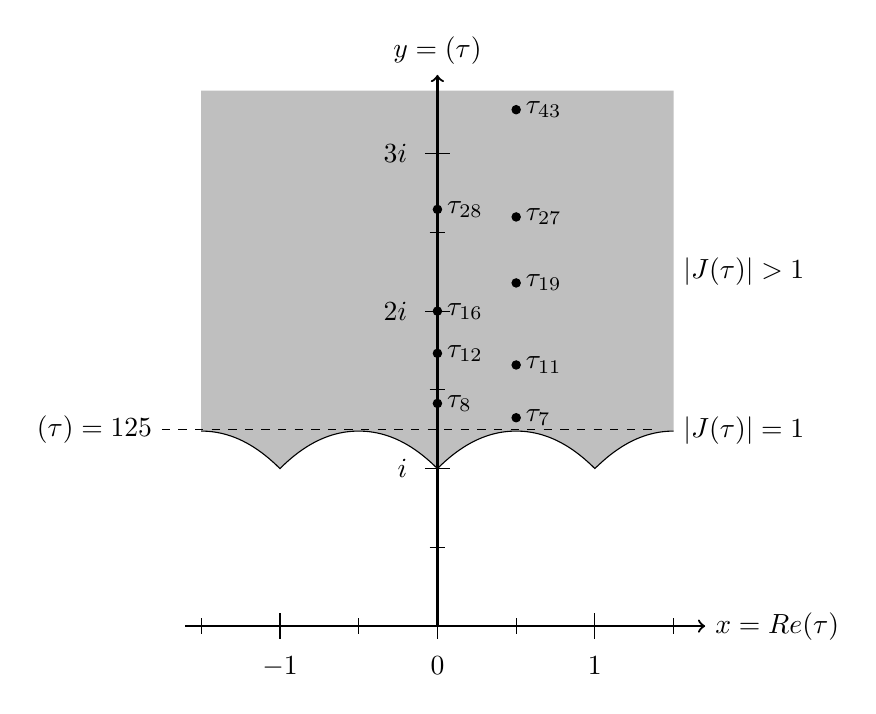
\begin{tikzpicture}[x=2cm, y=2cm] \def\anzPunkte{127}
   \def\mypath{{0.087793*pow(abs(\x-round(\x)),4)+0.099371*pow(abs(\x-round(\x)),3)-1.118425*pow(abs(\x-round(\x)),2)+(abs(\x-round(\x)))+1}}
   \path[fill=lightgray] (-1.5,3.4) -- plot[samples=\anzPunkte,domain=-1.5:1.5] (\x,\mypath) -- (1.5,3.4) -- cycle;
   \draw[->,thick] (-1.6,0) -- (1.7,0) node[right] {$x=\operatorname{Re}(\tau)$};
   \draw[->,thick] (0,0) -- (0,3.5) node[above] {$y=\im(\tau)$};
   \foreach \c in {-1,0,1}{ \draw (\c,-.08) -- (\c,.08) node[below=12pt] {$\c$}; }
   \draw (-.08,1) -- (.08,1) node[left=12pt] {$i$};
   \foreach \c in {2,3} { \draw (-.08,\c) -- (.08,\c) node[left=12pt] {$\c i$}; }
   \foreach \c in {-1.5,-0.5,0.5,1.5}{ \draw (\c,-.05) -- (\c,.05); }
   \foreach \c in {0.5,1.5,2.5} { \draw (-.05,\c) -- (.05,\c); }
   \draw[dashed](-1.75,1.25)node[left]{$\im(\tau)=1\ko25$} -- (1.4,1.25) ;
   \draw plot[samples=\anzPunkte,domain=-1.5:1.5] (\x,\mypath)  node[right] {$|J(\tau)|=1$};
   \draw (1.5,2.25) node[right] {$|J(\tau)|>1$};
   \draw[fill=black] (0.0,1.414) circle (1.5pt) node[right] {$\tau_8$};
    \draw[fill=black] (0,1.732) circle (1.5pt) node[right] {$\tau_{12}$};
	\draw[fill=black] (0,2) circle (1.5pt) node[right] {$\tau_{16}$};
	\draw[fill=black] (0,2.646) circle (1.5pt) node[right] {$\tau_{28}$};
	\draw[fill=black] (0.5,1.323) circle (1.5pt) node[right] {$\tau_{7}$};
	\draw[fill=black] (0.5,1.658) circle (1.5pt) node[right] {$\tau_{11}$};
	\draw[fill=black] (0.5,2.179) circle (1.5pt) node[right] {$\tau_{19}$};
	\draw[fill=black] (0.5,2.598) circle (1.5pt) node[right] {$\tau_{27}$};
	\draw[fill=black] (0.5,3.279) circle (1.5pt) node[right] {$\tau_{43}$};
\end{tikzpicture} 
\caption{\en{The region with $\im(\tau)>1$ and $|J(\tau)|>1$ has been calculated with Mathematica and is colored gray here.\newline
Also depicted: The values of $\tau_N$ (cf.~Prop.~\ref{\en{EN}satztaun}) which will lead to a Chudnovsky type formula.
$\tau_{67}$ and $\tau_{163}$ are outside the depicted area, above $\tau_{43}.$}%
\de{Hier ist das Gebiet mit $\im(\tau)>1$ und $|J(\tau)|>1$ grau gefärbt, das mit Mathematica berechnet wurde.\newline
Außerdem sind die Werte $\tau_N$ (vgl.~Satz~\ref{\en{EN}satztaun}) eingezeichnet, die auf eine Formel zur Berechnung von $\pi$ führen werden.
$\tau_{67}$ und $\tau_{163}$ liegen oberhalb von $\tau_{43}$ außerhalb des dargestellten Bereichs.}}\label{\en{EN}abb1}
\end{figure}

\begin{proof}[\en{Proof of Theorem}\de{Beweis des Theorems}~\ref{\en{EN}omegastrich}]
\en{In Thm.~\ref{\en{EN}theonaeherJ} we proved that for all $\tau$ with $\im(\tau)>1\ko25$ it holds: $|J(\tau)|>1$.
From Prop.~\ref{\en{EN}satzkonv} we deduce absolute convergence of the hypergeometric function ${_2F_1}$ in the region $\im(\tau)>1\ko25$ using $|z|=\left|\frac 1 J\right|<1$.
The present proof of Thm.~\ref{\en{EN}omegastrich} follows \cite[ch.~2.3 and 2.5]{\en{EN}lit02}:}%
\de{In Thm.~\ref{\en{EN}theonaeherJ} haben wir bewiesen, dass $|J(\tau)|>1$ für alle $\tau$ mit $\im(\tau)>1\ko25$ gilt. Aus Satz~\ref{\en{EN}satzkonv} folgt dann mit $|z|=\left|\frac 1 J\right|<1$ die absolute Konvergenz der angegebenen hypergeometrischen Funktion ${_2F_1}$ im Bereich $\im(\tau)>1\ko25$. Der jetzt folgende Beweis des Theorems~\ref{\en{EN}omegastrich} orientiert sich an \cite[Kap.~2.3 und 2.5]{\en{EN}lit02}:}

\en{We proved in Prop.~\ref{\en{EN}satzbj} that $b(J)= J^{-\frac 1 4}\cdot(1-J)^{\frac 1 4}\cdot{_2F_1}\lk\frac{1}{12},\frac{5}{12};1;\frac 1 J\rk$ is a solution of the Picard Fuchs differential equation for $|J|>1$.
But we already know two independent solutions of this second order differential equation -- the two basic periods $\Omega_1$ and $\Omega_2$ of $L_J$.
The Picard-Lindelöf theorem tells us that the solution $b(J)$ can be written as a linear combination of these basic periods, i.e.~that there are two complex numbers $A$ and $B$ satisfying
$b(J)=A\cdot\Omega_1(J) + B\cdot \Omega_2(J)$.}%
\de{Wir haben in Satz~\ref{\en{EN}satzbj} bewiesen, dass $b(J)= J^{-\frac 1 4}\cdot(1-J)^{\frac 1 4}\cdot{_2F_1}\lk\frac{1}{12},\frac{5}{12};1;\frac 1 J\rk$ für $|J|>1$ eine Lösung der Picard-Fuchs-Differential"-gleichung ist.
Wir kennen aber bereits zwei unabhängige Lösungen dieser Differentialgleichung zweiter Ordnung -- nämlich die beiden Basisperioden $\Omega_1$ und $\Omega_2$ von $L_J$.
Hieraus folgt mit dem Satz von Picard-Lindelöf, dass man die Lösung $b(J)$ als Linearkombination dieser beiden Perioden schreiben kann, also dass es komplexe Zahlen $A$ und $B$ gibt, sodass
$b(J)=A\cdot\Omega_1(J) + B\cdot \Omega_2(J)$ ist.}

\pagebreak

\en{In Def.~\ref{\en{EN}definLJ} we see that the basic periods $(\Omega_1,\Omega_2)$ of $L_J$ can be written in the form $\mu(\tau)\cdot(1,\tau)$ with $\mu(\tau)=\sqrt{\frac{g_3(\tau)}{g_2(\tau)}}$. We will write $\mu$ in terms of $J$:
}%
\de{In Definition~\ref{\en{EN}definLJ} erkennen wir, dass man die Basisperioden $(\Omega_1,\Omega_2)$ von $L_J$ in der Form $\mu(\tau)\cdot(1,\tau)$ mit $\mu(\tau)=\sqrt{\frac{g_3(\tau)}{g_2(\tau)}}$ schreiben kann. Wir werden zunächst $\mu$ mit Hilfe der $J$-Funktion schreiben:}
\begin{align}
    \frac{27J}{J-1} &= \frac{27g_2^3}{\Delta\cdot\left(\frac{g_2^3}{\Delta}-1\right)} = \frac{27g_2^3}{g_2^3-\Delta} = \frac{27g_2^3}{g_2^3-\left(g_2^3-27g_3^2\right)} = \frac{g_2^3}{g_3^2}\nonumber\\
    \Longrightarrow~~\mu&=\sqrt{\frac{g_3}{g_2}} = \left(\frac{g_3^2}{g_2^2}\right)^{\frac 1 4} = \left(g_2\cdot \frac{g_3^2}{g_2^3}\right)^{\frac 1 4} = \left(g_2\cdot \frac{J-1}{27J}\right)^{\frac 1 4}\nonumber\\
    &=\left(\left(J\cdot\Delta\right)^{\frac 1 3}\cdot \frac{J-1}{27J}\right)^{\frac 1 4} = 27^{-\frac 1 4} \cdot J^{-\frac 1 6} \cdot \left(J-1\right)^{\frac 1 4} \cdot \Delta^\frac 1 {12}\label{\en{EN}mue}
\end{align}

\en{This proves the existence of complex numbers $A$ and $B$ with $b(J)=A\cdot\Omega_1+B\cdot\Omega_2=(A+B\tau)\cdot\mu$ and thus}%
\de{Also gibt es komplexe $A$ und $B$, sodass $b(J)=A\cdot\Omega_1+B\cdot\Omega_2=(A+B\tau)\cdot\mu$ und somit}
\begin{align*}
    J^{-\frac 1 4}\cdot(1-J)^{\frac 1 4}\cdot{_2F_1}\lk\frac{1}{12},\frac{5}{12};1;\frac 1 J\rk &=\left(A + B\tau\right)\cdot 27^{-\frac 1 4} \cdot J^{-\frac 1 6} \cdot \left(J-1\right)^{\frac 1 4} \cdot \Delta^\frac 1 {12}\\
    \Longrightarrow\quad J^{-\frac{1}{12}}\cdot\Delta^{-\frac 1 {12}}\cdot{_2F_1}\lk\frac{1}{12},\frac{5}{12};1;\frac 1 J\rk &= C + D\tau
\end{align*}
\en{for two complex $C$ and $D$. Here we included $27^{-\frac 1 4}$ into the new numbers $C$ and $D$.}%
\de{für passende komplexe Zahlen $C$ und $D$. Hierbei wurde der Faktor $27^{-\frac 1 4}$ in die neuen komplexen Zahlen $C$ und $D$ integriert.}


\en{First we calculate $D$: It holds $e^{2\pi i (\tau+1)}=e^{2\pi i \tau}\cdot e^{2\pi i}=e^{2\pi i \tau}$.
Then we deduce from the Fourier representations in Thm.~\ref{\en{EN}fouriertheorem}, that $E_4(\tau+1)=E_4(\tau)$ and $E_6(\tau+1)=E_6(\tau)$.
This yields (again with Thm.~\ref{\en{EN}fouriertheorem}), that $J(\tau+1)=J(\tau)$ and $\Delta(\tau+1)=\Delta(\tau)$.
This shows that the left hand side of the above equation is invariant under the transformation $\tau\mapsto\tau+1$.
Thus the right hand side must also be invariant under this transformation -- we obtain $D=0$.}%
\de{Um $D$ zu berechnen, bemerken wir zunächst, dass $e^{2\pi i (\tau+1)}=e^{2\pi i \tau}\cdot e^{2\pi i}=e^{2\pi i \tau}$ gilt.
Dann folgt mit den Darstellungen in Theorem~\ref{\en{EN}fouriertheorem}, dass $E_4(\tau+1)=E_4(\tau)$ und $E_6(\tau+1)=E_6(\tau)$ gilt.
Hieraus folgt (ebenfalls mit den Darstellungen aus Theorem~\ref{\en{EN}fouriertheorem}), dass $J(\tau+1)=J(\tau)$ und $\Delta(\tau+1)=\Delta(\tau)$ ist. Folglich ist die linke Seite dieser Gleichung invariant unter der Transformation $\tau\mapsto\tau+1$, also muss es auch die rechte Seite sein -- wir erhalten $D=0$.}

\en{We get the value of $C$ by calculating the limit $\tau\rightarrow i\infty$ (which is allowed since our solution holds in the whole region $\im(\tau)>1\ko25$). This limit implies $q=e^{2\pi i \tau}\rightarrow 0$.
But from Thm.~\ref{\en{EN}theonaeherJ} we get $|1728J|>\frac{0\ko737}{|q|}$, which implies $\frac{1}{J(\tau)}\rightarrow 0$.
Then Def.~\ref{\en{EN}defihyp} shows that ${_2F_1}\lk\frac{1}{12},\frac{5}{12};1;\frac 1 J\rk\rightarrow 1$.
From the representation of $J$ and $\Delta$ in Thm.~\ref{\en{EN}fouriertheorem} und from the Fourier series of $E_4$ in the same Thm.~\ref{\en{EN}fouriertheorem} we get:}%
\de{Den Wert von $C$ erhalten wir z.B., indem wir auf der linken Seite $\tau\rightarrow i\infty$ gehen lassen (das dürfen wir, weil diese Lösung im ganzen Bereich $\im(\tau)>1\ko25$ gilt) und somit $q=e^{2\pi i \tau}\rightarrow 0$.
Dort gilt allerdings nach Theorem~\ref{\en{EN}theonaeherJ}, dass $|1728J|>\frac{0\ko737}{|q|}$, also dass  $\frac{1}{J(\tau)}\rightarrow 0$ gilt
und somit aus Def.~\ref{\en{EN}defihyp} folgt, dass ${_2F_1}\lk\frac{1}{12},\frac{5}{12};1;\frac 1 J\rk\rightarrow 1$.
Somit gilt wegen der Darstellung von $J$ und $\Delta$ aus Theorem~\ref{\en{EN}fouriertheorem} und wegen der dort befindlichen Darstellung von $E_4$:}
\begin{align*}
C&=\lim_{\tau\rightarrow i\infty}\left(J(\tau)\cdot\Delta(\tau)\right)^{-\frac 1 {12}}
= \lim_{\tau\rightarrow i\infty}\left(\frac{(2\pi)^{12}}{1728}\cdot E_4(\tau)^3\right)^{-\frac 1 {12}}\\
&=\left(\frac{(2\pi)^{12}}{12^3}\cdot 1\right)^{-\frac 1 {12}} = \frac{12^{\frac 1 4}}{2\pi}
\end{align*}
\en{This yields}\de{Schließlich erhalten wir}
$${_2F_1}\lk\frac{1}{12},\frac{5}{12};1;\frac 1 {J(\tau)}\rk = \frac{\sqrt[4]{12}}{2\pi}\cdot J(\tau)^{\frac{1}{12}}\cdot\Delta(\tau)^{\frac 1 {12}}$$
\en{where we recognize the equation from Thm.~\ref{\en{EN}omegastrich} because of $\tilde\omega_1 = \Delta(\tau)^{\frac 1 {12}}$.}%
\de{und erkennen darin wegen $\tilde\omega_1 = \Delta(\tau)^{\frac 1 {12}}$ die zu beweisende Gleichung.}
\end{proof}
